% !TEX root = ../pdf/lsr.tex
% [There are multiple lsr.tex files, but the one in ../pdf is the usual one]


\chapter{Basic programming~\label{ch:scripting}}

\begin{quote}
{\it Machine dreams hold a special vertigo.} \\
\hspace*{2cm}-- William Gibson
\end{quote}
%, Count Zero (1986

\noindent
Up to this point in the book I've tried hard to avoid using the word ``programming'' too much because -- at least in my experience -- it's a word that can cause a lot of fear. For one reason or another, programming (like mathematics and statistics) is often perceived by people on the ``outside'' as a black art, a magical skill that can be learned only by some kind of super-nerd. I think this is a shame. It's certainly true that advanced programming is a very specialised skill: several different skills actually, since there's quite a lot of different kinds of programming out there. However, the {\it basics} of programming aren't all that hard, and you can accomplish a lot of very impressive things just using those basics. 

With that in mind, the goal of this chapter is to discuss a few basic programming concepts and how to apply them in \R. However, before I do, I want to make one further attempt to point out just how non-magical programming really is, via one very simple observation: {\it you already know how to do it}. Stripped to its essentials, programming is nothing more (and nothing less) than the process of writing out a bunch of instructions that a computer can understand. To phrase this slightly differently, when you write a computer program, you need to write it in a \keyterm{programming language} that the computer knows how to interpret. \R\ is one such language. Although I've been having you type all your commands at the command prompt, and all the commands in this book so far have been shown as if that's what I were doing, it's also quite possible (and as you'll see shortly, shockingly easy) to write a program using these \R\ commands. In other words, if this is the first time reading this book, then you're only one short chapter away from being able to legitimately claim that you can program in \R, albeit at a beginner's level.    



\section{Scripts\label{sec:scripts}}


Computer programs come in quite a few different forms: the kind of program that we're mostly interested in from the perspective of everyday data analysis using \R\ is known as a \keyterm{script}. The idea behind a script is that, instead of typing your commands into the \R\ console one at a time, instead you write them all in a text file. Then, once you've finished writing them and saved the text file, you can get \R\ to execute all the commands in your file by using the \rtext{source()} function. In a moment I'll show you exactly how this is done, but first I'd better explain why you should care.


\SUBSECTION{Why use scripts?}

Before discussing scripting and programming concepts in any more detail, it's worth stopping to ask why you should bother. After all, if you look at the \R\ commands that I've used everywhere else this book, you'll notice that they're all formatted as if I were typing them at the command line. Outside this chapter you won't actually see any scripts. Do not be fooled by this. The reason that I've done it that way is purely for pedagogical reasons. My goal in this book is to teach statistics and to teach \R. To that end, what {\it I've} needed to do is chop everything up into tiny little slices: each section tends to focus on one kind of statistical concept, and only a smallish number of \R\ functions. As much as possible, I want you to see what each function does in isolation, one command at a time. By forcing myself to write everything as if it were being typed at the command line, it imposes a kind of discipline on me: it {\it prevents} me from piecing together lots of commands into one big script. From a teaching (and learning) perspective I think that's the right thing to do... but from a {\it data analysis} perspective, it is not. When you start analysing real world data sets, you will rapidly find yourself needing to write scripts.


To understand why scripts are so very useful, it may be helpful to consider the drawbacks to typing commands directly at the command prompt. The approach that we've been adopting so far, in which you type commands one at a time, and \R\ sits there patiently in between commands, is referred to as the \keyterm{interactive} style. Doing your data analysis this way is rather like having a conversation ... a very annoying conversation between you and your data set, in which you and the data aren't directly speaking to each other, and so you have to rely on \R\ to pass messages back and forth. This approach makes a lot of sense when you're just trying out a few ideas: maybe you're trying to figure out what analyses are sensible for your data, or maybe just you're trying to remember how the various \R\ functions work, so you're just typing in a few commands until you get the one you want. In other words, the interactive style is very useful as a tool for exploring your data. However, it has a number of drawbacks:
\begin{itemize}
\item {\it It's hard to save your work effectively}. You can save the workspace, so that later on you can load any variables you created.  You can save your plots as images. And you can even save the history or copy the contents of the \R\ console to a file. Taken together, all these things let you create a reasonably decent record of what you did. But it does leave a lot to be desired. It seems like you ought to be able to save a single file that \R\ could use (in conjunction with your raw data files) and reproduce everything (or at least, everything interesting) that you did during your data analysis.

\item {\it It's annoying to have to go back to the beginning when you make a mistake.} Suppose you've just spent the last two hours typing in commands. Over the course of this time you've created lots of new variables and run lots of analyses. Then suddenly you realise that there was a nasty typo in the first command you typed, so all of your later numbers are wrong. Now you have to fix that first command, and then spend another hour or so combing through the \R\ history to try and recreate what you did.


\item {\it You can't leave notes for yourself}. Sure, you can scribble down some notes on a piece of paper, or even save a Word document that summarises what you did. But what you really want to be able to do is write down an English translation of your \R\ commands, preferably right ``next to'' the commands themselves. That way, you can look back at what you've done and actually remember what you were doing. In the simple exercises we've engaged in so far, it hasn't been all that hard to remember what you were doing or why you were doing it, but only because everything we've done could be done using only a few commands, and you've never been asked to reproduce your analysis six months after you originally did it! When your data analysis starts involving hundreds of variables, and requires quite complicated commands to work, then you really, really need to leave yourself some notes to explain your analysis to, well, yourself. 

\item {\it It's nearly impossible to reuse your analyses later, or adapt them to similar problems}. Suppose that, sometime in January, you are handed a difficult data analysis problem. After working on it for ages, you figure out some really clever tricks that can be used to solve it. Then, in September, you get handed a really similar problem. You can sort of remember what you did, but not very well. You'd like to have a clean record of what you did last time, how you did it, and why you did it the way you did. Something like that would really help you solve this new problem.

\item{\it  It's hard to do anything except the basics.} There's a nasty side effect of these problems. Typos are inevitable. Even the best data analyst in the world makes a lot of mistakes. So the chance that you'll be able to string together dozens of correct \R\ commands in a row are very small. So unless you have some way around this problem, you'll never really be able to do anything other than simple analyses. 

\item {\it It's difficult to share your work other people.} Because you don't have this nice clean record of what \R\ commands were involved in your analysis, it's not easy to share your work with other people. Sure, you can send them all the data files you've saved, and your history and console logs, and even the little notes you wrote to yourself, but odds are pretty good that no-one else will really understand what's going on (trust me on this: I've been handed lots of random bits of output from people who've been analysing their data, and it makes very little sense unless you've got the original person who did the work sitting right next to you explaining what you're looking at)
\end{itemize}

Ideally, what you'd like to be able to do is something like this\ldots Suppose you start out with a data set \rtext{myrawdata.csv}. What you want is a single document -- let's call it \rtext{mydataanalysis.R} -- that stores all of the commands that you've used in order to do your data analysis. Kind of similar to the \R\ history but much more focused. It would only include the commands that you want to keep for later. Then, later on, instead of typing in all those commands again, you'd just tell \R\ to run all of the commands that are stored in \rtext{mydataanalysis.R}. Also, in order to help you make sense of all those commands, what you'd want is the ability to add some notes or {\it comments} within the file, so that anyone reading the document for themselves would be able to understand what each of the commands actually does. But these comments wouldn't get in the way: when you try to get \R\ to run \rtext{mydataanalysis.R} it would be smart enough would recognise that these comments are for the benefit of humans, and so it would ignore them. Later on you could tweak a few of the commands inside the file (maybe in a new file called \rtext{mynewdatanalaysis.R}) so that you can adapt an old analysis to be able to handle a new problem. And you could email your friends and colleagues a copy of this file so that they can reproduce your analysis themselves. 

In other words, what you want is a {\it script}.


\SUBSECTION{Our first script}

\begin{figure}[t]
\begin{center}
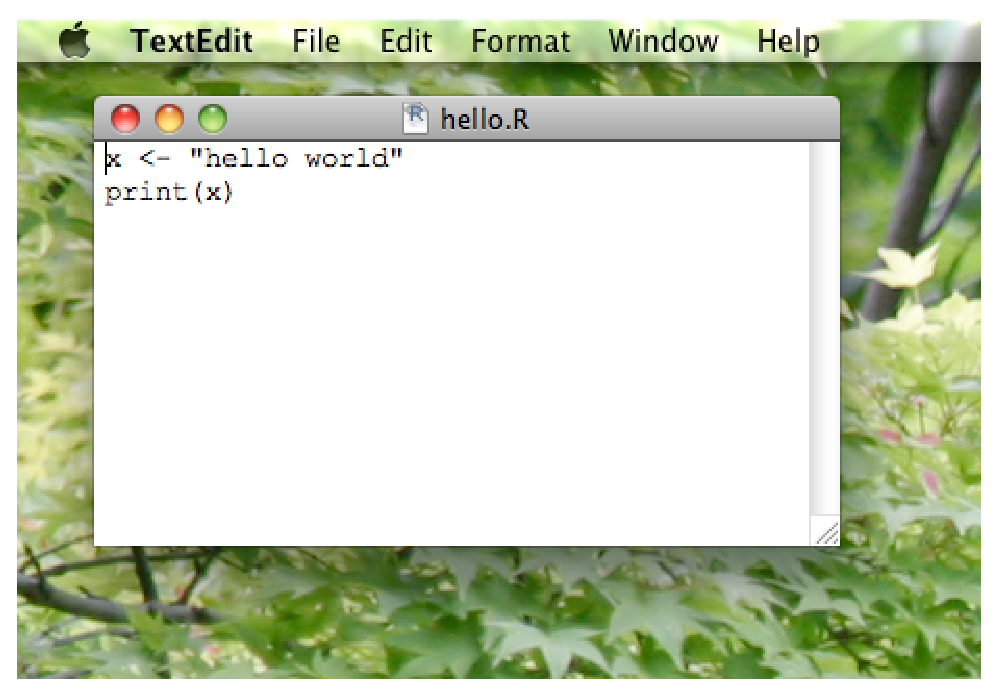
\epsfig{file = ../img/scripting/script.eps, clip=true,width = 10cm}
\caption{A screenshot showing the \filename{hello.R} script if you open in using the default text editor (TextEdit) on a Mac. Using a simple text editor like TextEdit on a Mac or Notepad on Windows isn't actually the best way to write your scripts, but it is the simplest. More to the point, it highlights the fact that a script really is just an ordinary text file.}
\label{fig:script}
\HR
\end{center}
\end{figure}

Okay then. Since scripts are so terribly awesome, let's write one. To do this, open up a simple text editing program, like TextEdit (on a Mac) or Notebook (on Windows). Don't use a fancy word processing program like Microsoft Word or OpenOffice: use the simplest program you can find. Open a new text document, and type some \R\ commands, hitting enter after each command. Let's try using \rtext{x <- "hello world"} and \rtext{print(x)} as our commands. Then save the document as \filename{hello.R}, and remember to save it as a plain text file: don't save it as a word document or a rich text file. Just a boring old plain text file. Also, when it asks you {\it where} to save the file, save it to whatever folder you're using as your working directory in \R. At this point, you should be looking at something like Figure~\ref{fig:script}. And if so, you have now successfully written your first \R\ program. Because I don't want to take screenshots for every single script, I'm going to present scripts using extracts formatted as follows:

\scriptname{hello.R}
\begin{script}
x <- "hello world"
print(x)
\end{script}
The line at the top is the filename, and not part of the script itself. Below that, you can see the two \R\ commands that make up the script itself. Next to each command I've included the line numbers. You don't actually type these into your script, but a lot of text editors (including the one built into Rstudio that I'll show you in a moment) will show line numbers, since it's a very useful convention that allows you to say things like ``line 1 of the script creates a new variable, and line 2 prints it out''. 

So how do we run the script? Assuming that the \filename{hello.R} file has been saved to your working directory, then you can run the script using the following command:
\begin{rblock1}
> @usr{source( "hello.R" )}
\end{rblock1}
If the script file is saved in a different directory, then you need to specify the path to the file, in exactly the same way that you would have to when loading a data file using \rtext{load()}. In any case, when you type this command, \R\ opens up the script file: it then reads each command in the file in the same order that they appear in the file, and executes those commands in that order. The simple script that I've shown above contains two commands. The first one creates a variable \rtext{x} and the second one prints it on screen. So, when we run the script, this is what we see on screen:
\begin{rblock1}
> @usr{source( "hello.R" )}
[1] "hello world"
\end{rblock1}
If we inspect the workspace using a command like \rtext{who()} or \rtext{objects()}, we discover that \R\ has created the new variable \rtext{x} within the workspace, and not surprisingly \rtext{x} is a character string containing the text \rtext{"hello world"}. And just like that, you've written your first program \R. It really is that simple. 



\begin{figure}[t]
\begin{center}
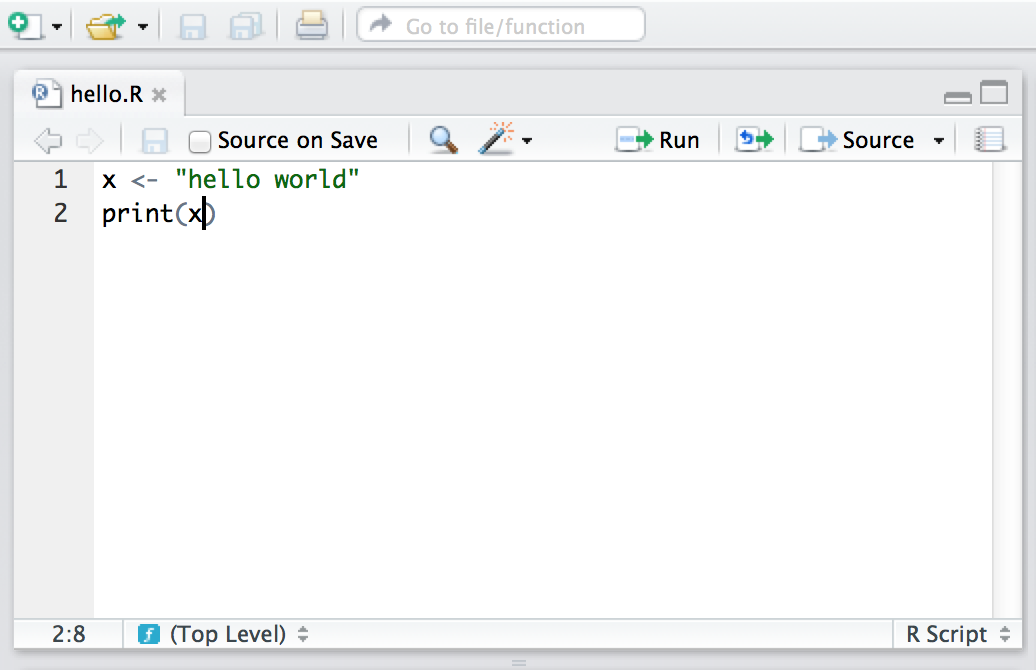
\epsfig{file = ../img/scripting/helloworld.eps,clip=true, width = 12cm}
\caption{A screenshot showing the \filename{hello.R} script open in Rstudio. Assuming that you're looking at this document in colour, you'll notice that the ``hello world'' text is shown in green. This isn't something that you do yourself: that's Rstudio being helpful. Because the text editor in Rstudio ``knows'' something about how \R\ commands work, it will highlight different parts of your script in different colours. This is useful, but it's not actually part of the script itself.}
\label{fig:script2}
\HR
\end{center}
\end{figure}


\SUBSECTION{Using Rstudio to write scripts}

In the example above I assumed that you were writing your scripts using a simple text editor. However, it's usually more convenient to use a text editor that is specifically designed to help you write scripts. There's a lot of these out there, and experienced programmers will all have their own personal favourites. For our purposes, however, we can just use the one built into Rstudio. To create new script file in R studio, go to the ``File '' menu, select the ``New'' option, and then click on ``R script''. This will open a new window within the ``source'' panel. Then you can type the commands you want (or \keyterm{code} as it is generally called when you're typing the commands into a script file) and save it when you're done. The nice thing about using Rstudio to do this is that it automatically changes the colour of the text to indicate which parts of the code are comments and which are parts are actual \R\ commands (these colours are called \keyterm{syntax highlighting}, but they're not actually part of the file -- it's just Rstudio trying to be helpful. To see an example of this, let's open up our \filename{hello.R} script in Rstudio. To do this, go to the ``File'' menu again, and select ``Open...''. Once you've opened the file, you should be looking at something like Figure~\ref{fig:script2}. As you can see (if you're looking at this book in colour) the character string ``hello world'' is highlighted in green.

Using Rstudio for your text editor is convenient for other reasons too. Notice in the top right hand corner of Figure~\ref{fig:script2} there's a little button that reads ``Source''? If you click on that, Rstudio will construct the relevant \rtext{source()} command for you, and send it straight to the \R\ console. So you don't even have to type in the \rtext{source()} command, which actually I think is a great thing, because it really bugs me having to type all those extra keystrokes every time I want to run my script. Anyway, Rstudio provide several other convenient little tools to help make scripting easier, but I won't discuss them here.\FOOTNOTE{Okay, I lied. Sue me. One of the coolest features of Rstudio is the support for {\it R Markdown}, which lets you embed R code inside a Markdown document, and you can automatically publish your R Markdown to the web on Rstudio's servers. If you're the kind of nerd interested in this sort of thing, it's really nice. And, yes, since I'm also that kind of nerd, of course I'm aware that iPython notebooks do the same thing and that \R\ just nicked their idea. So what? It's still cool. And anyway, this book isn't called {\it Learning Statistics with Python} now, is it? Hm. Maybe I should write a Python version...}


\SUBSECTION{Commenting your script}

When writing up your data analysis as a script, one thing that is generally a good idea is to include a lot of comments in the code. That way, if someone else tries to read it (or if you come back to it several days, weeks, months or years later) they can figure out what's going on. As a beginner, I think it's especially useful to comment thoroughly, partly because it gets you into the habit of commenting the code, and partly because the simple act of typing in an explanation of what the code does will help you keep it clear in your own mind what you're trying to achieve. To illustrate this idea, consider the following script:

\scriptname{itngscript.R}
\begin{script}
@cmt|# A script to analyse nightgarden.Rdata_
@cmt|#  author: Dan Navarro_
@cmt|#  date: 22/11/2011_

@cmt|# Load the data, and tell the user that this is what we're_
@cmt|# doing. Note that this assumes the nightgarden data file_ 
@cmt|# is in the working directory._
cat( "loading data from nightgarden.Rdata...\n" )
load( "nightgarden.Rdata" )

@cmt|# Create a cross tabulation and print it out:_
cat( "tabulating data...\n" )
itng.table <- table( speaker, utterance )
print( itng.table )
\end{script}
Firstly, as you can see from this extract I've done a tiny bit of syntax highlighting here, greying out the comments a bit so that you can visually distinguish between the commands that \R\ will execute and the comments which it it will ignore. Secondly, notice that I've gone a bit overboard with my commenting: at the top of the script I've explained the purpose of the script, who wrote it, and when it was written. Then, throughout the script file itself I've added a lot of comments explaining what each section of the code actually does. In real life people don't tend to comment this thoroughly, but the basic idea is a very good one: you really do want your script to explain itself.  Nevertheless, as you'd expect \R\ completely ignores all of the commented parts. When we run this script, this is what we see on screen:
\begin{rblock1}
> @usr{source( "itngscript.R" )}
loading data from nightgarden.Rdata...
tabulating data...
             utterance
speaker       ee onk oo pip
  makka-pakka  0   2  0   2
  tombliboo    1   0  1   0
  upsy-daisy   0   2  0   2
\end{rblock1}
Even here, notice that the script announces its behaviour. The first two lines of the output tell us a lot about what the script is actually doing behind the scenes (the code do to this corresponds to the two \rtext{cat()} commands on lines 8 and 12 of the script). It's usually a pretty good idea to do this, since it helps ensure that the output makes sense when the script is executed. 

\SUBSECTION{Differences between scripts and the command line}

For the most part, commands that you insert into a script behave in exactly the same way as they would if you typed the same thing in at the command line. The one major exception to this is that if you want a variable to be printed on screen, you need to explicitly tell \R\ to print it. You can't just type the name of the variable. For example, our original \rtext{hello.R} script produced visible output. The following script does not:

\scriptname{silenthello.R}
\begin{script}
x <- "hello world"
x
\end{script}
It {\it does} still create the variable \rtext{x} when you \rtext{source()} the script, but it won't print anything on screen. 

However, apart from the fact that scripts don't use ``auto-printing'' as it's called, there aren't a lot of differences in the underlying mechanics. There are a few stylistic differences though. For instance, if you want to load a package at the command line, you would generally use the \rtext{library()} function. If you want do to it from a script, it's conventional to use \rtext{require()} instead. The two commands are basically identical, the only difference being that if the package doesn't exist, \rtext{require()} produces a warning whereas \rtext{library()} gives you an error. Stylistically, what this means is that if the \rtext{require()} command fails in your script, \R\ will boldly continue on and try to execute the rest of the script. Often that's what you'd like to see happen, so it's better to use \rtext{require()}. Clearly, however, you can get by just fine using the \rtext{library()} command for everyday usage.


\SUBSECTION{Done!}

At this point, you've learned the basics of scripting. You are now officially allowed to say that you can program in \R, though you probably shouldn't say it too loudly. There's a {\it lot} more to learn, but nevertheless, if you can write scripts like these then what you are doing is in fact basic programming. The rest of this chapter is devoted to introducing some of the key commands that you need in order to make your programs more powerful; and to help you get used to thinking in terms of scripts, for the rest of this chapter I'll write up most of my extracts as scripts.


\section{Loops\label{sec:loops}}

The description I gave earlier for how a script works was a tiny bit of a lie. Specifically, it's not necessarily the case that \R\ starts at the top of the file and runs straight through to the end of the file. For all the scripts that we've seen so far that's exactly what happens, and unless you insert some commands to explicitly alter how the script runs, that is what will {\it always} happen. However, you actually have quite a lot of flexibility in this respect. Depending on how you write the script, you can have \R\ repeat several commands, or skip over different commands, and so on. This topic is referred to as \keyterm{flow control}, and the first concept to discuss in this respect is the idea of a \keyterm{loop}. The basic idea is very simple: a loop is a block of code (i.e., a sequence of commands) that \R\ will execute over and over again until some termination criterion is met. Looping is a very powerful idea. There are three different ways to construct a loop in \R, based on the \rtext{while}, \rtext{for} and \rtext{repeat} functions. I'll only discuss the first two in this book.

\SUBSECTION{The \rtext{while} loop}

A \rtext{while} loop is a simple thing. The basic format of the loop looks like this:
\begin{verbatim}
     while ( CONDITION ) {
        STATEMENT1
        STATEMENT2
        ETC
     }
\end{verbatim} 
The code corresponding to \textsc{condition} needs to produce a logical value, either \rtext{TRUE} or \rtext{FALSE}. Whenever \R\ encounters a \rtext{while} statement, it checks to see if the \textsc{condition} is \rtext{TRUE}. If it is, then \R\ goes on to execute all of the commands inside the curly brackets, proceeding from top to bottom as usual. However, when it gets to the bottom of those statements, it moves back up to the \rtext{while} statement. Then, like the mindless automaton it is, it checks to see if the \textsc{condition} is \rtext{TRUE}. If it is, then \R\ goes on to execute all ... well, you get the idea. This continues endlessly until at some point the \textsc{condition} turns out to be \rtext{FALSE}. Once that happens, \R\ jumps to the bottom of the loop (i.e., to the \rtextverb#}# character), and then continues on with whatever commands appear next in the script.

To start with, let's keep things simple, and use a \rtext{while} loop to calculate the smallest multiple of 17 that is greater than or equal to 1000. This is a very silly example since you can actually calculate it using simple arithmetic operations, but the point here isn't to do something novel. The point is to show how to write a \rtext{while} loop. Here's the script:

\scriptname{whileexample.R}
\begin{script}
x <- 0
while ( x < 1000 ) {
  x <- x + 17
}
print( x )
\end{script}
When we run this script, \R\ starts at the top and creates a new variable called \rtext{x} and assigns it a value of 0. It then moves down to the loop, and ``notices'' that the condition here is \rtext{x < 1000}. Since the current value of \rtext{x} is zero, the condition is true, so it enters the body of the loop (inside the curly braces). There's only one command here\FOOTNOTE{As an aside: if there's only a single command that you want to include inside your loop, then you don't actually need to bother including the curly braces at all. However, until you're comfortable programming in \R\ I'd advise {\it always} using them, even when you don't have to.} which instructs \R\ to increase the value of \rtext{x} by 17. \R\ then returns to the top of the loop, and rechecks the condition. The value of \rtext{x} is now 17, but that's still less than 1000, so the loop continues. This cycle will continue for a total of 59 iterations, until finally \rtext{x} reaches a value of 1003 (i.e., $59 \times 17 = 1003$). At this point, the loop stops, and \R\ finally reaches line 5 of the script, prints out the value of \rtext{x} on screen, and then halts. Let's watch:
\begin{rblock1}
> @usr{source( "whileexample.R" )}
[1] 1003
\end{rblock1}
Truly fascinating stuff.

\SUBSECTION{The \rtext{for} loop~\label{sec:for}} 

The \rtext{for} loop is also pretty simple, though not quite as simple as the \rtext{while} loop. The basic format of this loop goes like this:
\begin{verbatim}
     for ( VAR in VECTOR ) {
        STATEMENT1
        STATEMENT2
        ETC
     }
\end{verbatim} 
In a \rtext{for} loop, \R\ runs a fixed number of iterations. We have a \textsc{vector} which has several elements, each one corresponding to a possible value of the variable \textsc{var}. In the first iteration of the loop, \textsc{var} is given a value corresponding to the first element of \textsc{vector}; in the second iteration of the loop \textsc{var} gets a value corresponding to the second value in \textsc{vector}; and so on. Once we've exhausted all of the values in \textsc{vector}, the loop terminates and the flow of the program continues down the script. 

Once again, let's use some very simple examples. Firstly, here is a program that just prints out the word ``hello'' three times and then stops:

\scriptname{forexample.R}
\begin{script}
for ( i in 1:3 ) {
  print( "hello" )
}
\end{script}
This is the simplest example of a \rtext{for} loop. The vector of possible values for the \rtext{i} variable just corresponds to the numbers from 1 to 3. Not only that, the body of the loop doesn't actually depend on \rtext{i} at all. Not surprisingly, here's what happens when we run it:
\begin{rblock1}
> @usr{source( "forexample.R" )}
[1] "hello"
[1] "hello"
[1] "hello"
\end{rblock1}
However, there's nothing that stops you from using something non-numeric as the vector of possible values, as the following example illustrates. This time around, we'll use a character vector to control our loop, which in this case will be a vector of \rtext{words}. And what we'll do in the loop is get \R\ to convert the word to upper case letters, calculate the length of the word, and print it out. Here's the script: 

\scriptname{forexample2.R}
\begin{script}
@cmt|#the words_
words <- c("it","was","the","dirty","end","of","winter")

@cmt|#loop over the words_
for ( w in words ) {

  w.length <- nchar( w )     @cmt|# calculate the number of letters_
  W <- toupper( w )          @cmt|# convert the word to upper case letters_
  msg <- paste( W, "has", w.length, "letters" )   @cmt|# a message to print_
  print( msg )               @cmt|# print it_
  
}
\end{script}
And here's the output:
\begin{rblock1}
> @usr{source( "forexample2.R" )}
[1] "IT has 2 letters"
[1] "WAS has 3 letters"
[1] "THE has 3 letters"
[1] "DIRTY has 5 letters"
[1] "END has 3 letters"
[1] "OF has 2 letters"
[1] "WINTER has 6 letters"
\end{rblock1}
Again, pretty straightforward I hope.

\SUBSECTION{A more realistic example of a loop}

To give you a sense of how you can use a loop in a more complex situation, let's write a simple script to simulate the progression of a mortgage. Suppose we have a nice young couple who borrow \$300000 from the bank, at an annual interest rate of 5\%. The mortgage is a 30 year loan, so they need to pay it off within 360 months total. Our happy couple decide to set their monthly mortgage payment at \$1600 per month. Will they pay off the loan in time or not? Only time will tell.\FOOTNOTE{Okay, fine. This example is still a bit ridiculous, in three respects. Firstly, the bank absolutely will not let the couple pay less than the amount required to terminate the loan in 30 years. Secondly, a constant interest rate of 30 years is hilarious. Thirdly, you can solve this much more efficiently than through brute force simulation. However, we're not exactly in the business of being realistic or efficient here.} Or, alternatively, we could simulate the whole process and get \R\ to tell us. The script to run this is a fair bit more complicated. 

\scriptname{mortgage.R}
\begin{script}
@cmt|# set up_
month <- 0  @cmt|# count the number of months_
balance <- 300000 @cmt|# initial mortgage balance_
payments <- 1600 @cmt|# monthly payments_
interest <- 0.05  @cmt|# 5% interest rate per year_
total.paid <- 0 @cmt|# track what you've paid the bank_

@cmt|# convert annual interest to a monthly multiplier_
monthly.multiplier <- (1+interest) ^ (1/12)

@cmt|# keep looping until the loan is paid off..._
while ( balance > 0 ) {
  
  @cmt|# do the calculations for this month_
  month <- month + 1  @cmt|# one more month_
  balance <- balance * monthly.multiplier  @cmt|# add the interest_
  balance <- balance - payments  @cmt|# make the payments_
  total.paid <- total.paid + payments @cmt|# track the total paid_
  
  @cmt|# print the results on screen_
  cat( "month", month, ": balance", round(balance), "\n")
  
} @cmt|# end of loop_

@cmt|# print the total payments at the end_
cat("total payments made", total.paid, "\n" )
\end{script}
To explain what's going on, let's go through it carefully. In the first block of code (lines 2-6) all we're doing is specifying all the variables that define the problem. The loan starts with a \rtext{balance} of \$300,000 owed to the bank on \rtext{month} zero, and at that point in time the \rtext{total.paid} money is nothing. The couple is making monthly \rtext{payments} of \$1600, at an annual \rtext{interest} rate of 5\%. Next, on line 9, we convert the annual percentage interest into a monthly multiplier. That is, the number that you have to multiply the current balance by each month in order to produce an annual interest rate of 5\%. An annual interest rate of 5\% implies that, if no payments were made over 12 months the balance would end up being $1.05$ times what it was originally, so the {\it annual} multiplier is $1.05$. To calculate the monthly multiplier, we need to calculate the 12th root of 1.05 (i.e., raise 1.05 to the power of 1/12). We store this value in as the \rtext{monthly.multiplier} variable, which as it happens corresponds to a value of about 1.004. All of which is a rather long winded way of saying that the {\it annual} interest rate of 5\% corresponds to a {\it monthly} interest rate of about 0.4\%. 

Anyway... all of that is really just setting the stage. It's not the interesting part of the script. The interesting part (such as it is) is the loop which unfolds over lines 12-23. The \rtext{while} statement on line 12 tells \R\ that it needs to keep looping until the \rtext{balance} reaches zero (or less, since it might be that the final payment of \$1600 pushes the balance below zero). Then, inside the body of the loop, we have two different blocks of code. In the first bit, on lines 15-18, we do all the number crunching. Firstly we increase the value \rtext{month} by 1 (on line 15). Next, the bank charges the interest (on line 16), so the \rtext{balance} goes up. Then, the couple makes their monthly payment (on line 17) and the \rtext{balance} goes down. Finally, we keep track of the total amount of money that the couple has paid so far, by adding the \rtext{payments} to the running tally (on line 18). After having done all this number crunching, we tell \R\  (on line 21) to issue the couple with a very terse monthly statement, which just indicates how many months they've been paying the loan and how much money they still owe the bank. Which is rather rude of us really. I've grown attached to this couple and I really feel they deserve better than that. But, that's banks for you.

In any case, the key thing here is the tension between the increase in \rtext{balance} on line 16 and the decrease on line 17. As long as the decrease is bigger, then the balance will eventually drop to zero and the loop will eventually terminate. If not, the loop will continue forever! This is actually very bad programming on my part: I really should have included something to force \R\ to stop if this goes on too long. However, I haven't shown you how to evaluate ``if'' statements yet, so we'll just have to hope that the author of the book has rigged the example so that the code actually runs. Hm. I wonder what the odds of that are? Anyway, assuming that the loop does eventually terminate, there's one last line of code (line 26) that prints out the total amount of money that the couple handed over to the bank over the lifetime of the loan. 

Now that I've explained everything in the script in tedious detail, let's run it and see what happens:
\begin{rblock1}
> @usr{source( "mortgage.R" )}
month 1 : balance 299622 
month 2 : balance 299243 
month 3 : balance 298862 
month 4 : balance 298480 
month 5 : balance 298096 

BLAH BLAH BLAH

month 352 : balance 4806 
month 353 : balance 3226 
month 354 : balance 1639 
month 355 : balance 46 
month 356 : balance -1554 
total payments made 569600 
\end{rblock1}
So our nice young couple have paid off their \$300,000 loan in just 4 months shy of the 30 year term of their loan, at a bargain basement price of \$568,046 (since  569600 - 1554 = 568046). A happy ending!


\section{Conditional statements\label{sec:if}}

A second kind of flow control that programming languages provide is the ability to evaluate \keyterm{conditional statements}. Unlike loops, which can repeat over and over again, a conditional statement only executes once, but it can switch between different possible commands depending on a \textsc{condition} that is specified by the programmer. The power of these commands is that they allow the program itself to make choices, and in particular, to make different choices depending on the context in which the program is run. The most prominent of example of a conditional statement is the \rtext{if} statement, and the accompanying \rtext{else} statement. The basic format of an \rtext{if} statement in \R\ is as follows:
\begin{verbatim}
     if ( CONDITION ) {
        STATEMENT1
        STATEMENT2
        ETC
     }
\end{verbatim}
And the execution of the statement is pretty straightforward. If the \textsc{condition} is true, then \R\ will execute the statements contained in the curly braces. If the \textsc{condition} is false, then it dose not. If you want to, you can extend the \rtext{if} statement to include an \rtext{else} statement as well, leading to the following syntax:
\begin{verbatim}
     if ( CONDITION ) {
        STATEMENT1
        STATEMENT2
        ETC
     } else {
        STATEMENT3
        STATEMENT4
        ETC
     }     
\end{verbatim}
As you'd expect, the interpretation of this version is similar. If the \textsc{condition} is true, then the contents of the first block of code (i.e., \textsc{statement1}, \textsc{statement2}, \textsc{etc}) are executed; but if it is false, then the contents of the second block of code (i.e., \textsc{statement3}, \textsc{statement4}, \textsc{etc}) are executed instead. 

To give you a feel for how you can use \rtext{if} and \rtext{else} to do something useful, the example that I'll show you is a script that prints out a different message depending on what day of the week you run it. We can do this making use of some of the tools that we discussed in Section~\ref{sec:dates}. Here's the script:

\scriptname{ifelseexample.R}
\begin{script}
@cmt|# find out what day it is..._
today <- Sys.Date()       @cmt|# pull the date from the system clock_
day <- weekdays( today )  @cmt|# what day of the week it is_

@cmt|# now make a choice depending on the day..._
if ( day == "Monday" ) {
  print( "I don't like Mondays" )
} else {
  print( "I'm a happy little automaton" )
}
\end{script}
Since today happens to be a Tuesday, when I run the script here's what happens:
\begin{rblock1}
> @usr{source( "ifelseexample.R" )}
[1] "I'm a happy little automaton"
\end{rblock1}

There are other ways of making conditional statements in \R. In particular, the \rtext{ifelse()} function and the \rtext{switch()} functions can be very useful in different contexts. However, my main aim in this chapter is to briefly cover the very basics, so I'll move on.





\section{Writing functions\label{sec:functions}}

In this section I want to talk about functions again. Functions were introduced in Section~\ref{sec:usingfunctions}, but you've learned a lot about \R\ since then, so we can talk about them in more detail. In particular, I want to show you how to create your own. To stick with the same basic framework that I used to describe loops and conditionals, here's the syntax that you use to create a function:
\begin{verbatim}
     FNAME <- function ( ARG1, ARG2, ETC ) {
        STATEMENT1
        STATEMENT2
        ETC
        return( VALUE )
     }
\end{verbatim} 
What this does is create a function with the name \textsc{fname}, which has arguments \textsc{arg1}, \textsc{arg2} and so forth. Whenever the function is called, \R\ executes the statements in the curly braces, and then outputs the contents of \textsc{value} to the user. Note, however, that \R\ does not execute the commands inside the function in the workspace. Instead, what it does is create a temporary local environment: all the internal statements in the body of the function are executed there, so they remain invisible to the user. Only the final results in the \textsc{value} are returned to the workspace.

To give a simple example of this, let's create a function called \rtext{quadruple()} which multiplies its inputs by four. In keeping with the approach taken in the rest of the chapter, I'll use a script to do this:

\scriptname{functionexample.R}
\begin{script}
quadruple <- function(x) {
  y <- x*4
  return(y)
} 
\end{script}
When we run this script, as follows
\begin{rblock1}
> @usr{source( "functionexample.R" )}
\end{rblock1}
nothing appears to have happened, but there is a new object created in the workspace called \rtext{quadruple}. Not surprisingly, if we ask \R\ to tell us what kind of object it is, it tells us that it is a function:
\begin{rblock1}
> @usr{class( quadruple )}
[1] "function"
\end{rblock1}
And now that we've created the \rtext{quadruple()} function, we can call it just like any other function 
And if I want to store the output as a variable, I can do this:
\begin{rblock1}
> @usr{my.var <- quadruple(10)}
> @usr{print(my.var)}
[1] 40
\end{rblock1}
An important thing to recognise here is that the two internal variables that the \rtext{quadruple()} function makes use of, \rtext{x} and \rtext{y}, stay internal. That is, if we inspect the contents of the workspace, 
\begin{rblock1}
> @usr{who()}
   --- Name ---   --- Class ---
   my.var         numeric      
   quadruple      function  
\end{rblock1}
we see only the \rtext{quadruple()} function itself, as well as the \rtext{my.var} variable that we just created. 

Now that we know how to create our own functions in \R, it's probably a good idea to talk a little more about some of the other properties of functions that I've been glossing over. To start with, let's take this opportunity to type the name of the function at the command line without the parentheses:
\begin{rblock1}
> @usr{quadruple}
function(x) {
  y <- x*4
  return(y)
}
\end{rblock1}
As you can see, when you type the name of a function at the command line, \R\ prints out the underlying source code that we used to define the function in the first place. In the case of the \rtext{quadruple()} function, this is quite helpful to us -- we can read this code and actually see what the function does. For other functions, this is less helpful, as we saw back in Section~\ref{sec:usingfunctions} when we tried typing \rtext{citation} rather than \rtext{citation()}. 

\SUBSECTION{Function arguments revisited~\label{sec:dotsargument}}

Okay, now that we are starting to get a sense for how functions are constructed, let's have a look at two, slightly more complicated functions that I've created. The source code for these functions is contained within the \filename{functionexample2.R} and \filename{functionexample3.R} scripts. Let's start by looking at the first one:

\scriptname{functionexample2.R}
\begin{script}
pow <- function( x, y = 1) {
  out <- x^y  @cmt|# raise x to the power y_
  return( out )
}
\end{script}
and if we type \rtext{source("functionexample2.R")} to load the \rtext{pow()} function into our workspace, then we can make use of it. As you can see from looking at the code for this function, it has two arguments \rtext{x} and \rtext{y}, and all it does is raise \rtext{x} to the power of \rtext{y}. For instance, this command
\begin{rblock1}
> @usr{pow( x=3, y=2 )}
[1] 9
\end{rblock1}
calculates the value of $3^2$. The interesting thing about this function isn't what it does, since \R\ already has has perfectly good mechanisms for calculating powers. Rather, notice that when I defined the function, I specified \rtext{y=1} when listing the arguments? That's the default value for \rtext{y}. So if we enter a command without specifying a value for \rtext{y}, then the function assumes that we want \rtext{y=1}:
\begin{rblock1}
> @usr{pow( x=3 )}
[1] 3
\end{rblock1}
However, since I didn't specify any default value for \rtext{x} when I defined the \rtext{pow()} function, we always need to input a value for \rtext{x}. If we don't \R\ will spit out an error message.

So now you know how to specify default values for an argument. The other thing I should point out while I'm on this topic is the use of the \rtext{...} argument. The \rtext{...} argument is a special construct in \R\ which is only used within functions. It is used as a way of matching against multiple user inputs: in other words, \rtext{...} is used as a mechanism to allow the user to enter as many inputs as they like. I won't talk at all about the low-level details of how this works at all, but I will show you a simple example of a function that makes use of it. To that end, consider the following script:

\scriptname{functionexample3.R}
\begin{script}
doubleMax <- function( ... ) {  
  max.val <- max( ... )   @cmt|# find the largest value in ... _
  out <- 2 * max.val      @cmt|# double it_ 
  return( out )
}
\end{script}
When we type \rtext{source("functionexample3.R")}, \R\ creates the \rtext{doubleMax()} function. You can type in as many inputs as you like. The \rtext{doubleMax()} function identifies the largest value in the inputs, by passing all the user inputs to the \rtext{max()} function, and then doubles it. For example:
\begin{rblock1}
> @usr{doubleMax( 1,2,5 )}
[1] 10
\end{rblock1}

\SUBSECTION{There's more to functions than this}

There's a lot of other details to functions that I've hidden in my description in this chapter. Experienced programmers will wonder exactly how the ``scoping rules'' work in \R,\FOOTNOTE{Lexical scope.} or want to know how to use a function to create variables in other environments\FOOTNOTE{The \rtextsmall{assign()} function.}, or if function objects can be assigned as elements of a list\FOOTNOTE{Yes.} and probably hundreds of other things besides. However, I don't want to have this discussion get too cluttered with details, so I think it's best -- at least for the purposes of the current book -- to stop here.





\section{Implicit loops\label{sec:vectorised}}

There's one last topic I want to discuss in this chapter. In addition to providing the explicit looping structures via \rtext{while} and \rtext{for}, \R\ also provides a collection of functions for \keyterm{implicit loops}. What I mean by this is that these are functions that carry out operations very similar to those that you'd normally use a loop for. However, instead of typing out the whole loop, the whole thing is done with a single command. The main reason why this can be handy is that -- due to the way that \R\ is written -- these implicit looping functions are usually about to do the same calculations much faster than the corresponding explicit loops. In most applications that beginners might want to undertake, this probably isn't very important, since most beginners tend to start out working with fairly small data sets and don't usually need to undertake extremely time consuming number crunching. However, because you often see these functions referred to in other contexts, it may be useful to very briefly discuss a few of them.

The first and simplest of these functions is \rtext{sapply()}. The two most important arguments to this function are \rtext{X}, which specifies a vector containing the data, and \rtext{FUN}, which specifies the name of a function that should be applied to each element of the data vector. The following example illustrates the basics of how it works:
\begin{rblock1}
> @usr{words <- c("along", "the", "loom", "of", "the", "land")}
> @usr{sapply( X = words, FUN = nchar )}
along   the  loom    of   the  land 
    5     3     4     2     3     4 
\end{rblock1}
Notice how similar this is to the second example of a \rtext{for} loop in Section~\ref{sec:for}. The \rtext{sapply()} function has implicitly looped over the elements of \rtext{words}, and for each such element applied the \rtext{nchar()} function to calculate the number of letters in the corresponding word.

The second of these functions is \rtext{tapply()}, which has three key arguments. As before \rtext{X} specifies the data, and \rtext{FUN} specifies a function. However, there is also an \rtext{INDEX} argument which specifies a grouping variable.\FOOTNOTE{Or a list of such variables.} What the \rtext{tapply()} function does is loop over all of the different values that appear in the \rtext{INDEX} variable. Each such value defines a group: the \rtext{tapply()} function constructs the subset of \rtext{X} that corresponds to that group, and then applies the function \rtext{FUN} to that subset of the data. This probably sounds a little abstract, so let's consider a specific example, using the \filename{nightgarden.Rdata} file that we used in Chapter~\ref{ch:datahandling}. 
\begin{rblock1}
> @usr{gender <- c( "male","male","female","female","male" )}
> @usr{age <- c( 10,12,9,11,13 )}
> @usr{tapply( X = age, INDEX = gender, FUN = mean )}
  female     male 
10.00000 11.66667
\end{rblock1}
In this extract, what we're doing is using \rtext{gender} to define two different groups of people, and using their \rtext{ages} as the data. We then calculate the \rtext{mean()} of the ages, separately for the males and the females. A closely related function is \rtext{by()}. It actually does the same thing as \rtext{tapply()}, but the output is formatted  a bit differently. This time around the three arguments are called \rtext{data}, \rtext{INDICES} and \rtext{FUN}, but they're pretty much the same thing. An example of how to use the \rtext{by()} function is shown in the following extract:
\begin{rblock1}
> @usr{by( data = age, INDICES = gender, FUN = mean )}
gender: female
[1] 10
------------------------------------------------------------------------- 
gender: male
[1] 11.66667
\end{rblock1}
The \rtext{tapply()} and \rtext{by()} functions are quite handy things to know about, and are pretty widely used. However, although I do make passing reference to the \rtext{tapply()} later on, I don't make much use of them in this book.

Before moving on, I should mention that there are several other functions that work along similar lines, and have suspiciously similar names: \rtext{lapply}, \rtext{mapply}, \rtext{apply}, \rtext{vapply}, \rtext{rapply} and \rtext{eapply}. However, none of these come up anywhere else in this book, so all I wanted to do here is draw your attention to the fact that they exist.






\section{Summary}

In this chapter I talked about several key programming concepts, things that you should know about if you want to start converting your simple scripts into full fledged programs:

\begin{itemize}
\item Writing and using scripts (Section~\ref{sec:scripts}).
\item Using loops (Section~\ref{sec:loops}) and implicit loops (Section~\ref{sec:vectorised}).
\item Making conditional statements (Section~\ref{sec:if})
\item Writing your own functions (Section~\ref{sec:functions})
\end{itemize}

\noindent
As always, there are {\it lots} of things I'm ignoring in this chapter. It takes a lot of work to become a proper programmer, just as it takes a lot of work to be a proper psychologist or a proper statistician, and this book is certainly not going to provide you with all the tools you need to make that step. However, you'd be amazed at how much you can achieve using only the tools that I've covered up to this point. Loops, conditionals and functions are very powerful things, especially when combined with the various tools discussed in Chapters~\ref{ch:introR}, \ref{ch:mechanics} and \ref{ch:datahandling}. Believe it or not, you're off to a pretty good start just by having made it to this point. If you want to keep going, there are (as always!) several other books you might want to look at. One that I've read and enjoyed is  ``A first course in statistical programming with R'' \cite{Braun2007}, but quite a few people have suggested to me that ``The art of programming with R'' \cite{Matloff2011} is worth the effort too. 



